\documentclass{report}

% Add missing packages
\usepackage{csquotes}
\usepackage{tocbasic}
\usepackage{fancyhdr}
\usepackage{bookmark}
\usepackage{listings}
\usepackage{enumitem}
\lstset{
  breaklines=true, % Active le retour à la ligne automatique
  basicstyle=\ttfamily\small, % Définit le style de base pour le code
  columns=fullflexible, % Pour éviter d'espacer les caractères
}
% \usepackage{lipsum}
% \usepackage{natbib}
\usepackage{hyperref}
\usepackage{float}
\usepackage[nottoc]{tocbibind} 
\usepackage[backend=biber,style=ieee,sorting=ynt]{biblatex} % for more plz click https://www.overleaf.com/learn/latex/Biblatex_citation_styles
\title{Report} %Titre du fichier

\addbibresource{references.bib} % Imports bibliography file
\begin{document}

%----------- Informations du rapport ---------
\titre{Multi-Physics Modeling} %Titre du rapport
\UE{Project-based TU} %Nom de la UE
% add image to the header


\enseignant{Christophe \textsc{Prud'Homme}\\
Joubine \textsc{Aghili}\\
Didier \textsc{Lemetayer}\\
Paul \textsc{Devigne}\\
Hanae \textsc{Mbarki}} %Nom de l'enseignant Abdoulaye Diallo
\eleves{Iman \textsc{Barkan} \\Job \textsc{Congo} } %Nom des élèves

%----------- Initialisation -------------------
        
\fairemarges%Afficher les marges
\fairepagedegarde%Créer la page de garde
\tabledesmatieres%Créer la table de matières

%------------ Corps du rapport ----------------


\section{Introduction} 

\subsection{Context}

In a world where energy efficiency and sustainable solutions are becoming increasingly important, our project, proposed in collaboration with BDRThermea, aims to explore new avenues in understanding and optimizing heat pumps. BDRThermea, a renowned player in the heating and cooling industry, is recognized for its deep commitment to sustainability and innovation. Founded on a mission of decarbonization, the company stands out for its proactive approach and ongoing investment in research and development. These systems, essential in heating and cooling applications, represent a fertile ground for technical and ecological innovation.

The concept of reverse engineering is at the heart of our approach. This technique, which involves deeply analyzing an existing system to deduce the underlying processes and parameters, is a powerful tool for improvement, innovation, and understanding. In our project, reverse engineering is applied to a heat pump compressor, a key component whose performance directly influences the overall efficiency of the system. The project benefits from close collaboration with the CAE \& Modeling team of BDRThermea, an R\&D division created in May 2022. This team is a group of specialists dedicated to helping develop innovative products and supporting all other hubs in four key areas: flow (fluid mechanics), multiphysics modeling, mechanics, and acoustics.

Our project focuses on a specific heat pump, whose steady-state performance has been previously tested and documented. However, although the pump itself has been modeled as a set of different components, the specific parameters of the compressor model remain unknown. Our main objective is therefore to fill this gap, by identifying and determining the missing parameters of the compressor model. This approach is essential not only for a complete understanding of the heat pump's operation but also for potential future improvements in its design and performance.

\subsection{Objectives}

The project aims to deepen understanding and optimization of heat pumps, focusing on the reverse engineering of key components, particularly the compressor. Our temporary roadmap revolves around several crucial steps, aiming to cover the entire modeling and analysis process.

\subsubsection{Modeling}

\begin{itemize}
    \item Understand the operation of heat pumps through bibliographic research and training. This initial phase is essential to acquire a solid foundation on which to base our subsequent work.

    \item Examine the technical documentation of compressors, focusing on the types of models already existing and their relevance to our project. This involves a thorough identification of the parameters used by BDRThermea for rotary compressors.
\end{itemize}

\subsubsection{Data Analysis}
\begin{itemize}

\item Data Extraction and Preparation: Clean and prepare the data from the entire heat pump system, eliminating errors or inconsistencies, to ensure the reliability of future analyses.

\item Parameter Calibration: Use test data to calibrate the parameters. This includes a sensitivity analysis to assess the impact of each input parameter on the performance of the heat pump. 

\item Cross-Validation: Compare the predictions of the calibrated model with a separate test dataset to verify the accuracy and reliability of the model.
\end{itemize}


\section{Operation of a Heat Pump}

\subsection{Basic Principles and Mechanisms}

The heat pump (HP) is a key element in the landscape of modern heating and cooling systems, characterized by its ability to transfer thermal energy from a low-temperature environment to a warmer medium. This technology defies the spontaneous transfer of heat, thus achieving a reversal of the natural flow of thermal energy. It stands out for its versatile role, serving as a heating system when it raises the temperature of a hot source, or acting as a refrigeration system by lowering the temperature of a cold source. The applications of the HP encompass various fields, from domestic air conditioners to industrial refrigerators.

The operation of an HP is similar to that of a refrigerator but with an inverted process for heating. Instead of extracting heat from a confined space to cool it, it captures heat from the external environment and transfers it inside a building. This process relies on the compression and expansion of a refrigerant gas, typically fluids like R407C, R410A, R134a, or R32, following precise thermodynamic cycles.

\subsection{Thermodynamic Cycle of an HP}

An HP operates according to a transformation cycle in four key stages, involving phase changes of the refrigerant:

Compression: In this phase, the refrigerant, initially in vapor form, is compressed, causing an increase in its pressure and temperature.

Condensation: The refrigerant, now at high temperature and pressure, passes through a condenser. Here, it releases its heat to the surrounding medium (e.g., the air in a room) and transforms into a liquid.

Expansion: After condensation, the high-pressure liquid passes through an expander. This step rapidly reduces the fluid's pressure, causing partial vaporization of it and resulting in a decrease in its temperature.

Evaporation: The refrigerant, now cold and partially vaporized, circulates through a heat exchanger (evaporator) located in the area to be cooled. By absorbing heat from this environment, the fluid completely evaporates, returning to the gaseous state.

\begin{figure}[H]
    \centering
    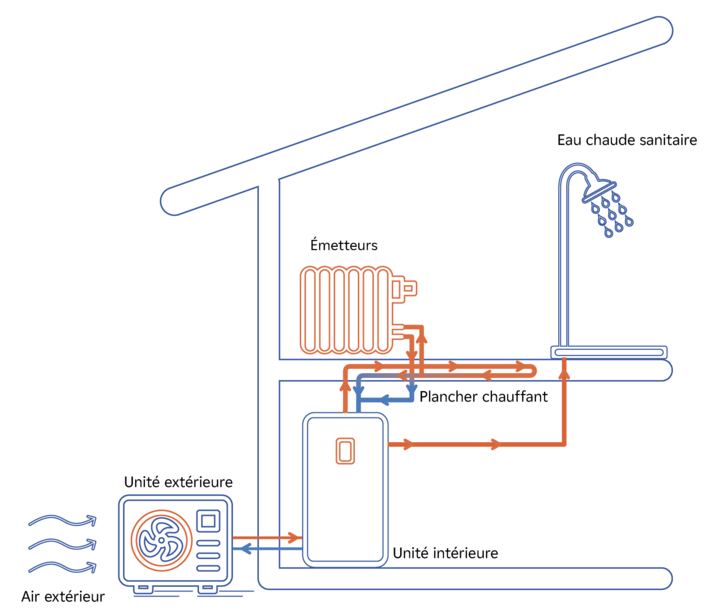
\includegraphics[width=0.75\textwidth]{images/fonctionnementpompe1.png}
    \caption{Operating diagram of HP \cite{schemafonctionnement}}
\end{figure}

\subsection{Key Components of the HP}

The circuit of the HP consists of four main components, each playing a vital role in the cycle:

The Condenser (Hot Source): Here, the refrigerant releases its heat to the secondary fluid (water, air, etc.), changing from gaseous to liquid state.

The Expander: This component reduces the pressure of the liquid refrigerant.

The Evaporator (Cold Source): Heat is absorbed from the secondary fluid, vaporizing the refrigerant.

The Compressor: Powered electrically or mechanically, it increases the pressure and temperature of the gaseous refrigerant.


\begin{figure}[H]
    \centering
    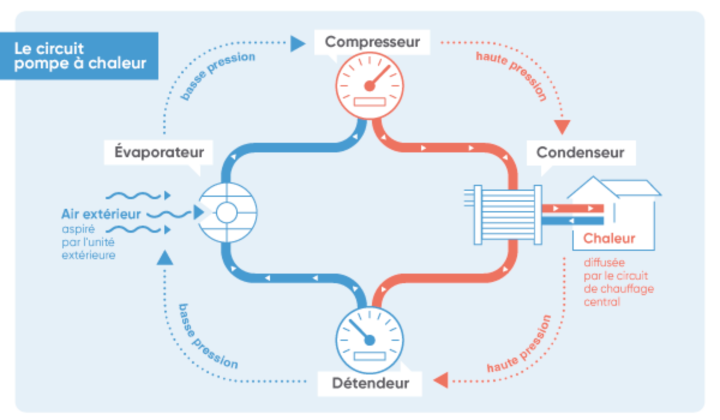
\includegraphics[width=0.75\textwidth]{images/fonctionnementpompe2.png}
    \caption{Component diagram of HP \cite{schemaComposant}}
\end{figure}

\section{Heat Pump Model}

\subsection{FMU Parameters}

In the modeling of the heat pump, various parameters are adjustable within their respective ranges. These parameters are crucial in simulating different operating conditions and analyzing the compressor's behavior under varied scenarios. The modifiable parameters include:


\begin{itemize}
    \item \textbf{x\_areaLeakage}: This parameter represents the total area through which leakage can occur within the compressor. The range from \(1 \times 10^{-8}\) to \(1 \times 10^{-6}\) square meters allows for the simulation of various leakage scenarios, which could be due to manufacturing imperfections, wear and tear, or design specifications. Leakage in a compressor can lead to a decrease in efficiency as it allows some of the refrigerant to escape the compression cycle, thus reducing the overall effectiveness of heat transfer.

    \item \textbf{x\_areaSuctionValve}: The area of the suction valve, adjustable between \(2 \times 10^{-6}\) and \(1 \times 10^{-3}\) square meters, plays a critical role in controlling the flow of refrigerant into the compressor. A larger valve area would typically allow more refrigerant to enter the compressor, potentially increasing the cooling capacity but also possibly affecting the efficiency and stability of the cycle. Conversely, a smaller valve area restricts the refrigerant flow, which could lead to lower power consumption but reduced cooling capacity.

    \item \textbf{x\_areaDischargeValve}: This parameter corresponds to the discharge valve area, which controls the flow of compressed refrigerant out of the compressor. The range from \(1 \times 10^{-7}\) to \(1 \times 10^{-4}\) square meters allows for the investigation of how the size of this valve affects the performance of the compressor. The discharge valve's area impacts the pressure within the compressor and influences the refrigerant's flow rate into the condenser, playing a crucial role in the efficiency and operational stability of the heat pump.
    \item \textbf{x\_relativeDeadSpace}: This parameter, varying between 0.001 and 0.1, reflects the relative dead space in the compressor. Dead space is the volume within the compressor where the refrigerant does not contribute to the compression process. This non-active volume can affect the efficiency of the compressor, as a larger dead space usually leads to lower efficiency. It represents the volume where the refrigerant is trapped and recompressed in each cycle without contributing to the cooling or heating process.
    \item \textbf{x\_driveEfficiency}: This parameter indicates the efficiency of the compressor's drive, spanning from 0.85 to 0.98. It represents how effectively the drive (usually an electric motor) converts electrical energy into mechanical energy to drive the compressor. Higher efficiency means that more of the electrical energy is converted into useful work for compressing the refrigerant, leading to a more efficient heat pump system overall. This parameter is especially critical in determining the overall energy consumption and performance of the heat pump.
\end{itemize}
The \textbf{x\_driveEfficiency} parameter is particularly significant as it corresponds to the efficiency of the electronic component regulating the compressor's frequency. Its dependency on the compressor frequency is modeled through a polynomial expression of the fourth order:
\begin{equation}
    x_\text{driveEfficiency} = a_5 \times \text{freq}^4 + a_4 \times \text{freq}^3 + a_3 \times \text{freq}^2 + a_2 \times \text{freq} + a_1
\end{equation}
where \text{freq} represents the compressor frequency, and \(a_1, a_2, a_3, a_4, a_5\) are the coefficients of the polynomial.

\subsection{FMU Inputs }
The Functional Mock-up Unit (FMU) for the heat pump model accepts several critical inputs, each playing a key role in simulating the system's behavior:

\begin{itemize}
    \item \textbf{u\_compressorFrequency (Compressor Frequency)}: This input represents the operating frequency of the compressor, measured in Hertz (Hz). The compressor frequency is a pivotal factor influencing the rate at which the refrigerant is compressed and circulated within the system. Higher frequencies typically increase the rate of compression and circulation, which can affect the cooling or heating capacity and the overall efficiency of the heat pump.

    \item \textbf{u\_VFlow (Volumetric Water Flow)}: This input specifies the volumetric flow rate of water through the heat pump, measured in cubic meters per second (m\(^3\)/s). The water flow rate is crucial in determining the heat transfer rate within the heat pump, as it affects how quickly heat is absorbed or released by the water circulating through the system.

    \item \textbf{u\_T\_water (Water Inlet Temperature)}: This input denotes the temperature of water entering the heat pump, measured in Kelvin (K). The inlet water temperature is an essential parameter in the heat pump's thermodynamic cycle, influencing the efficiency and the amount of heat absorbed or released during the process.

    \item \textbf{u\_T\_air (Air Inlet Temperature)}: This input measures the air temperature at the heat pump inlet, also in Kelvin (K). The air temperature is a critical environmental factor affecting the heat pump's performance, especially in air-source heat pumps, where the air serves as either the heat source or sink.
\end{itemize}

\subsection{FMU Outputs }
The outputs from the FMU provide insights into the performance and efficiency of the heat pump under simulated conditions:

\begin{itemize}
    \item \textbf{y\_T\_out (Water Outlet Temperature)}: This output reflects the temperature of water leaving the heat pump, measured in Kelvin (K). It is indicative of the heat pump's ability to transfer heat and is crucial for assessing the system's heating or cooling performance.

    \item \textbf{y\_heatPower (Thermal Power)}: This output, measured in Watts (W), represents the thermal power generated on the hot side of the heat pump. It indicates the rate at which the heat pump transfers heat, which is vital for evaluating its heating performance and efficiency.

    \item \textbf{y\_elecPower (Electrical Power Consumption)}: This output measures the electrical power consumption of the heat pump in Watts (W). It is a key indicator of the system's energy efficiency, representing the electrical energy required to operate the heat pump.

    \item \textbf{y\_COP (Coefficient of Performance)}: 

    The Coefficient of Performance is a critical output from the Functional Mock-up Unit (FMU), offering a dimensionless measure of the heat pump's efficiency. It is computed based on the thermodynamic principles governing the heat pump's operation. The COP varies depending on whether the heat pump is in cooling or heating mode, as the interest shifts between the cold and hot reservoirs. 
    The equation for COP is expressed as \cite{Chesser2021}:
    \begin{equation}
        COP = \frac{|Q|}{W}
    \end{equation}
    where:
    
    -\( Q \) represents the useful heat supplied (in heating mode) or removed (in cooling mode) by the system.
    
    -\( W \) is the net work input into the system for one cycle, which is always positive.
    
    The COP values for cooling and heating differ due to the distinct focus on either the cold or hot reservoir:
    
    -\textbf{Cooling COP}:
       In cooling mode, the COP calculates the efficiency in terms of the heat removed from the cold reservoir relative to the input work. It is defined as:
       \begin{equation}
           COP_{cooling} = \frac{|Q_C|}{W} = \frac{Q_C}{W}
       \end{equation}
       Here, \( Q_C \) is the heat absorbed from the cold reservoir.
    
    -\textbf{Heating COP}:
       Conversely, in heating mode, the COP is the ratio of the magnitude of heat delivered to the hot reservoir to the input work. Since the hot reservoir receives the heat extracted from the cold reservoir plus the input work, the heating COP is formulated as:
       \begin{equation}
           COP_{heating} = \frac{|Q_H|}{W} = \frac{Q_C + W}{W} = COP_{cooling} + 1
       \end{equation}
       Here, \( Q_H \) is the heat released to the hot reservoir, which is negative as per the convention in thermodynamics.
    
 
\end{itemize}

\subsection{Simulation of the FMU}
The \texttt{HeatPumpSimulator} class in Python offers a  framework for simulating the heat pump's performance using the FMU2Slave interface from the FMPy library. The class is designed to streamline the simulation process, allowing for a detailed analysis of the heat pump under various conditions. Its functionalities include:


\begin{itemize}
    \item \textbf{Initialization}: The constructor initializes the class with the FMU file name, simulation start and stop times, and the step size. It reads the model description from the FMU file using FMPy's \texttt{read\_model\_description} function. This step is crucial as it sets the stage for the entire simulation by loading the necessary model information and defining the simulation timeline.

    \item \textbf{FMU Preparation}: The \texttt{prepare\_fmu} method handles the extraction and preparation of the FMU file for simulation. It locates the FMU file within the notebook directory, creates an \texttt{unzip} directory for the extracted contents, and uses the \texttt{extract} function from FMPy to unpack the FMU. This method ensures that all necessary files and components of the FMU are accessible for the simulation.

    \item \textbf{Parameter Range Verification}: The \texttt{verify\_parameter\_ranges} method checks if the initial values of the simulation parameters are within their defined permissible ranges. This validation step is crucial for maintaining the integrity and accuracy of the simulation, ensuring that the parameters used are realistic and within expected bounds.

    \item \textbf{Timeout-Enabled Simulation}: The \texttt{simulate\_with\_timeout} method runs the simulation within a separate thread, allowing for a timeout mechanism. This approach prevents the simulation from running indefinitely in case of unresponsive scenarios or computational issues, thereby enhancing the robustness of the simulation framework.

    \item \textbf{Simulation Execution}:
        
    -The \texttt{simulate} method is the core of the simulation process. It instantiates an FMU slave using the model's GUID and model identifier, then sets up the simulation with the given start values.
        
        -The setup involves initializing the FMU for the experiment, setting the real values of the parameters, and then entering and exiting the initialization mode.
        
        -The \texttt{run\_simulation} sub-method then executes the simulation over the defined timeframe. It iterates through the simulation time, performing steps at each interval and collecting output values for each of the specified variables.
        
        -Exception handling is incorporated to ensure any errors during simulation are caught and handled appropriately, preventing crashes and providing meaningful error messages.

    \item \textbf{Data Collection and Analysis}:
        
        -As the simulation runs, data for each output variable (like \texttt{y\_T\_out}, \texttt{y\_heatPower}, \texttt{y\_elecPower}, \texttt{y\_COP}) is collected and stored in a dictionary format.
        
        -This data can be used for further analysis, such as plotting the results to visualize the performance of the heat pump over time. While the \texttt{plot\_results} method is a placeholder in the provided code, it can be implemented to generate graphs and charts for a more intuitive understanding of the simulation results.
\end{itemize}




\section{Data presentation}

The data represents the results of 85 tests carried out on a heat pump. The information is organised in columns with various characteristics recorded during the tests. After deleting incomplete results, there are 79 usable data items. Here is a general description of the data :

\textbf{General information:}
\begin{itemize}
    \item Date: Test date
    \item Test location :  Mertzwiller or Techneco
    \item ODU : Type of system (GP561)  
    \item P.H.E.: Model (B26Hx26)
    \item Réfrigérant : R32 
    \item Charge : 980 g
\end{itemize}

\textbf{Main features:}
\begin{itemize}
    \item Setpoint : run times in seconds.
    \item Frequency : Compressor frequency in Hz
    \item Water in : Water temperature at heat pump inlet °C
    \item Water out : Water temperature at heat pump outlet °C
    \item Flow : Water flow rate in m³/h
    \item Defrosts : Présence ou absence de dégivrage (yes/no)
    \item Current (max) : Maximum electrical current
    \item Power out : Heat pump thermal power in W
    \item Power in : Electrical power of the heat pump in W
    \item COP : coefficient of performance of the heat pump
\end{itemize}

\textbf{Additional features:}
\begin{itemize}
    \item Toshiba PCBs : Presence of Toshiba PCBs (yes/no)
    \item Toshiba PCBs : Presence of main board (yes/no)
    \item Pump : Presence of the pump (yes/no)
    \item Corrected COP : COP corrected according to certain conditions
    \item Remarks : Observations or specific notes
    \item rotation : rotation of heat pump in hz
\end{itemize}

\section{Calibration Algorithms}

\subsection{ Non-dominated Sorting Genetic Algorithm (NSGA-II)}
\subsubsection{Overview}
The NSGA-II (Non-Dominated Sorting Genetic Algorithm II) algorithm is an evolutionary technique 
developed for solving multi-objective optimisation problems. It was introduced by Kalyanmoy Deb, 
Amrit Pratap, Sameer Agarwal, and T. Meyarivan in 2002, as an improvement on the original NSGA.

The main objective of the NSGA-II algorithm is to find solutions that are not dominated by other 
solutions, by providing a set of optimal and balanced solutions in the objective space.


\subsubsection{NSGA-II algorithm stages}

The various stages in the general operation of the NSGA-II algorithm are as follows.
\begin{enumerate}[label=\arabic*.]
    \item Random creation of the first generation \(P_0\) of size \(N\), from the imposed search spaces.
    \item Creation of a set of children \(Q_t\) of size \(N\) by genetic operators such as selection, crossover, and mutation.
    \item Mixture of \(P_t\) and \(Q_t\): \(R_t = Q_t \cup P_t\).
    \item Calculation of all the boundaries \(F_i\) of \(R_t\) and addition into \(P_{t+1}\) until the size of \(P_{t+1}\) is equal to \(N\).
    \item Returns to 2.
\end{enumerate}


\begin{figure}[H]
    \centering
    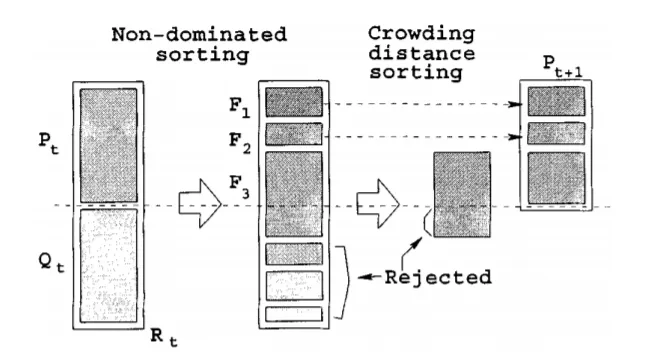
\includegraphics[width=0.75\textwidth]{images/nsga2_survival.png}
    \caption{ NSGA-II algorithm stages \cite{nsga2}}
\end{figure}



Non-dominated sorting: NSGA-II uses a non-dominated sorting technique to classify solutions into 
multiple edges, where solutions on the first edge are not dominated by any other solution, 
solutions on the second edge are dominated only by those on the first edge, and so on.


Crowding distance sorting : For each solution in the \(F_3\) front, the crowding distance is 
calculated by considering the values of the neighbouring criteria. More precisely, the crowding 
distance of a solution is the sum of the distances between neighbouring solutions on each of the 
criteria.

\subsection{Particle Swarm Optimization (PSO)}

\subsubsection{Overview}
Particle Swarm Optimization (PSO) is a computational method that optimizes a problem by iteratively improving a candidate solution with regard to a given measure of quality. PSO utilizes a swarm of particles, which are potential solutions, to probe the search space. Particles adjust their positions in the search space by following two essential components: the cognitive and social components.
Introduced by James Kennedy and Russel Eberhart in 1995 \cite{Pereira2011PSO}, PSO's inspiration stems from the social behavior patterns of animals such as bird flocking and fish schooling. These natural processes led to PSO being categorized under Swarm Intelligence and Artificial Life domains. The algorithm's strength lies in its simplicity and minimal need for parameterization.

\subsubsection{Algorithmic Principles}
The core of PSO lies in simulating the movements of a swarm of particles through the problem space. Each particle represents a potential solution to the optimization problem. The particles 'fly' through the problem space and adjust their positions based on their own experience and the experience of neighboring particles.

\paragraph{Particle Dynamics}
Each particle in the swarm has two main attributes:

- \textbf{Position} (\(x_i\)): Represents the current solution of the particle.

- \textbf{Velocity} (\(v_i\)): Dictates the direction and magnitude of the particle’s movement in the search space.

\paragraph{Position and Velocity Update}
\begin{figure}[H]
    \centering
    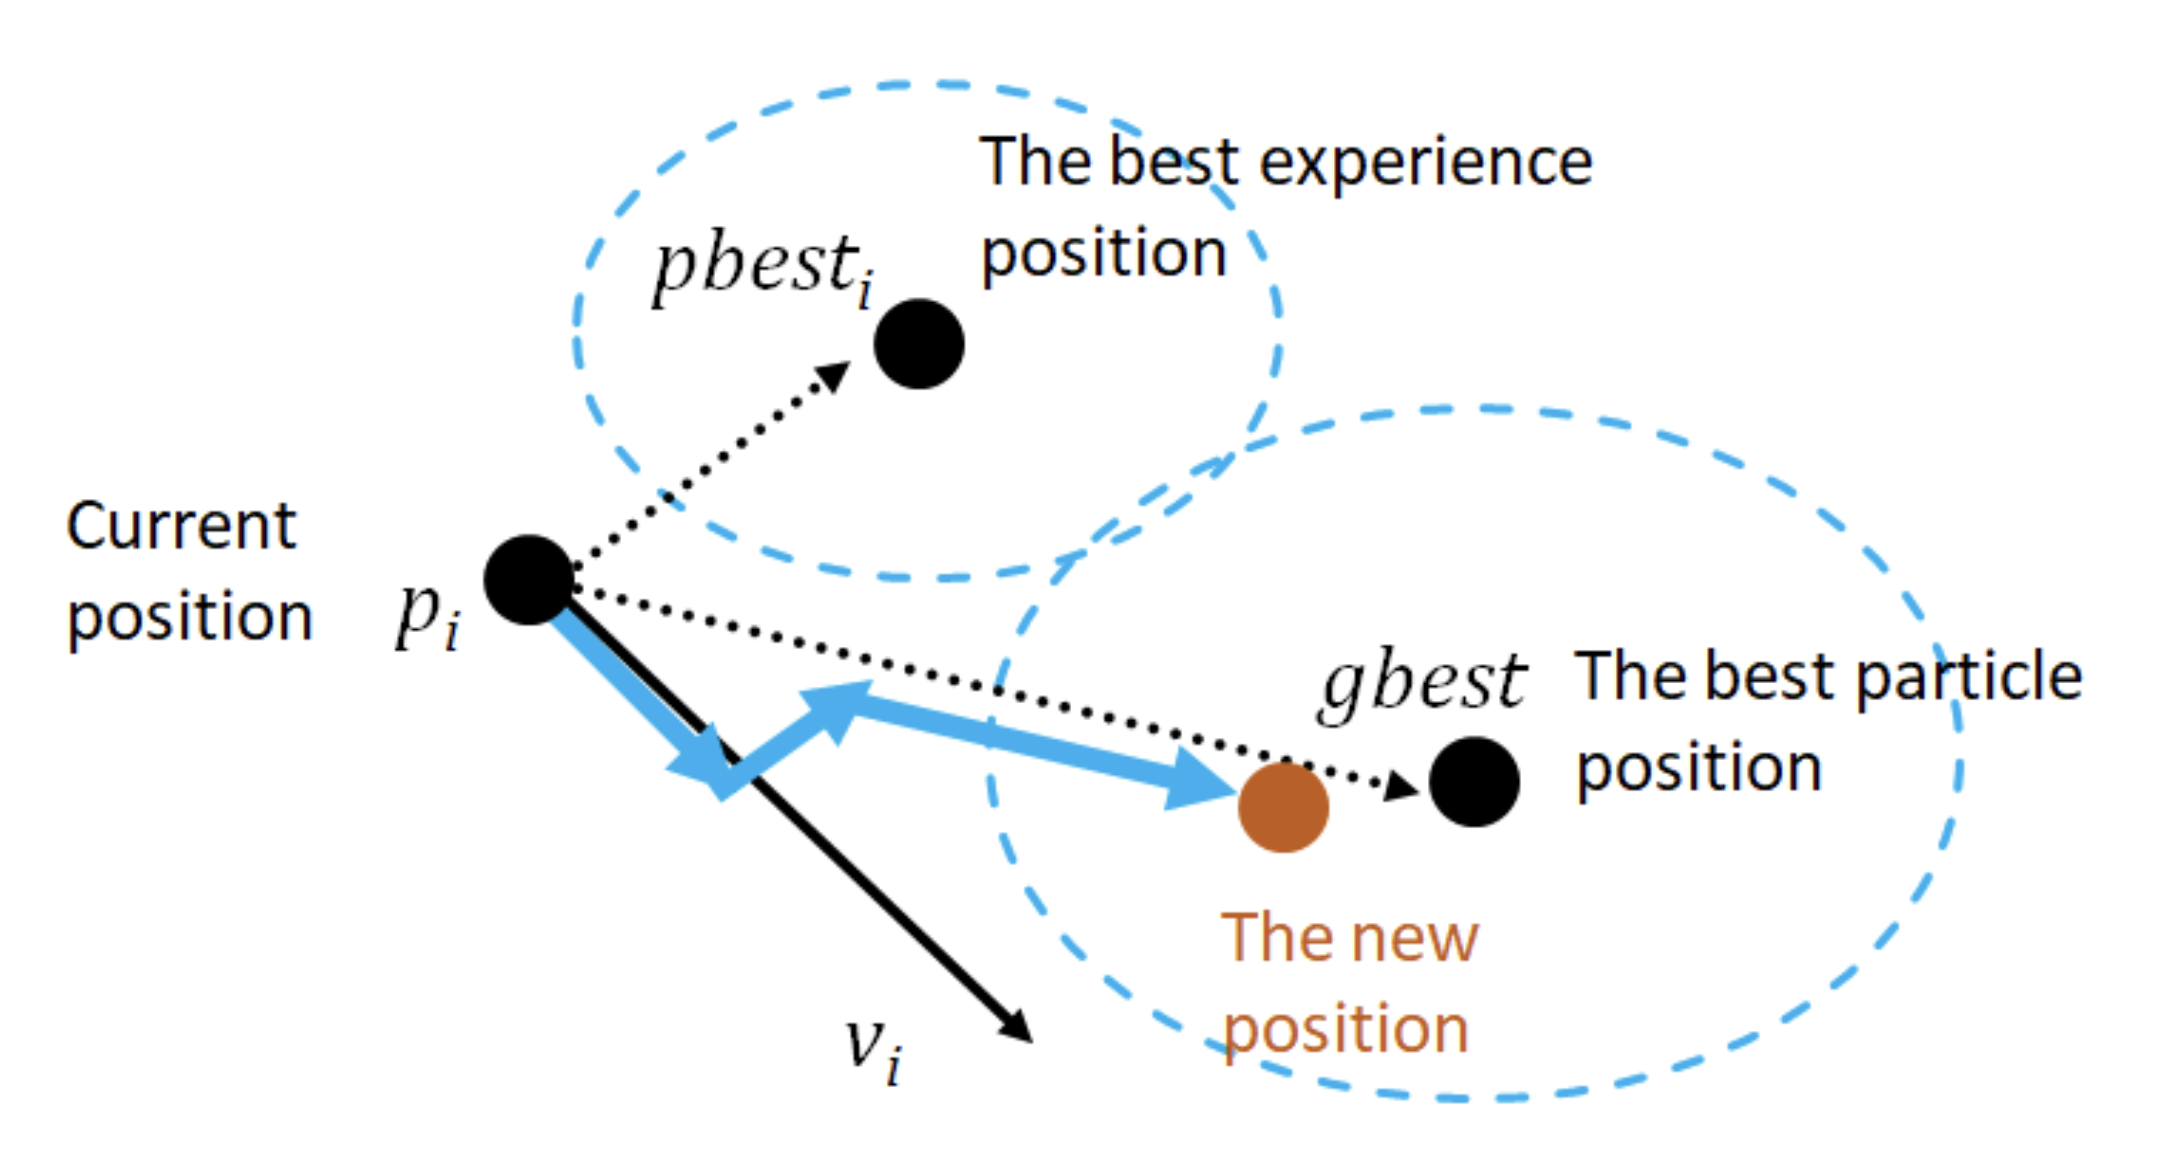
\includegraphics[width=0.75\textwidth]{images/pso-vectors.png}
    \caption{Position and Velocity Vectors \cite{BaeldungPSOImage}}
\end{figure}

The position and velocity of each particle are updated according to the following equations:

\begin{equation}
x_{i,d}(t+1) = x_{i,d}(t) + v_{i,d}(t+1)
\end{equation}
\begin{equation}
v_{i,d}(t+1) = v_{i,d}(t) + C_1 \cdot \text{Rnd}(0, 1) \cdot [p_{bi,d}(t) - x_{i,d}(t)] + C_2 \cdot \text{Rnd}(0, 1) \cdot [g_{b,d}(t) - x_{i,d}(t)]
\end{equation}
Where:

- \(x_{i,d}(t)\) and \(v_{i,d}(t)\) are the position and velocity of particle \(i\) in dimension \(d\) at iteration \(t\).

- \(C_1\) and \(C_2\) are cognitive and social acceleration constants.

- \text{Rnd}(0, 1) is a random number between 0 and 1.

- \(p_{bi,d}(t)\) is the best-known position of particle \(i\) in dimension \(d\).

- \(g_{b,d}(t)\) is the best-known position among all particles in the swarm.

\paragraph{Cognitive and Social Components}
\quad- The cognitive component (\(C_1\)) represents the particle's own experience. It is the knowledge of the particle's best position found so far.

- The social component (\(C_2\)) represents learning from the swarm’s experience, reflecting the best position found by any particle in the swarm.

\paragraph{Initialization and Control Parameters}
The initialization of the swarm is critical to the algorithm’s performance. Particles are typically placed randomly or uniformly within the problem space, with velocities often initialized to small random values. Key parameters in PSO include:

- Swarm size.

- Values of \(C_1\) and \(C_2\), which balance exploration and exploitation.

- Maximum iterations or convergence criteria.

\subsubsection{Pyswarm PSO Implementation}

The Particle Swarm Optimization algorithm, as implemented in the Pyswarm Python library \cite{pyswarmPSO}, is a method for finding optimal solutions to complex problems. The code is structured to utilize the PSO algorithm for calibration purposes, optimizing parameters based on a given objective function.

\paragraph{Initialization and Parameter Setting}

The function \texttt{pso} accepts the objective function (\texttt{func}), lower (\texttt{lb}) and upper (\texttt{ub}) bounds of the search space, and various PSO-specific parameters. The lower and upper bounds define the feasible region within which the particles can search for solutions.

Key parameters for the PSO include \texttt{swarmsize} (number of particles in the swarm), \texttt{omega} (inertia weight), \texttt{phip} (personal learning coefficient), and \texttt{phig} (global learning coefficient). These parameters govern the behavior and efficiency of the swarm.

\paragraph{Particle Dynamics}

Each particle in the swarm is represented by its position and velocity. The position (\(x_i\)) indicates the current solution of the particle, and the velocity (\(v_i\)) determines the particle's movement through the search space.

The position and velocity of each particle are updated iteratively based on their personal best position, the swarm's global best position, and random factors that encourage exploration. The update equations are as follows:

\begin{equation}
v_{i,d} = \omega \cdot v_{i,d} + \text{phip} \cdot \text{Rnd}(0, 1) \cdot (p_{bi,d} - x_{i,d}) + \text{phig} \cdot \text{Rnd}(0, 1) \cdot (g_{b,d} - x_{i,d})
\end{equation}
\begin{equation}
x_{i,d} = x_{i,d} + v_{i,d}
\end{equation}

\paragraph{Objective Function Evaluation}

The core of the optimization process involves evaluating the fitness of each particle using the objective function \texttt{func}. This function assesses the quality of each solution, guiding the swarm towards the most promising regions of the search space.

\subsubsection{Calibration using PSO}

The \texttt{line\_calibration} function implemented in our simulation notebook demonstrates the application of PSO for calibration. It optimizes parameters for each line in the input DataFrame \texttt{df\_input\_no\_defrost\_cal}, using the PSO algorithm to minimize the objective function.

\begin{itemize}
    \item The function iterates over each line of the DataFrame.
    \item For each line, PSO is executed by calling the \texttt{pso} function with the objective function and the bounds (\texttt{lb} and \texttt{ub}).
    \item The best solution (\texttt{xopt}) and the corresponding error (\texttt{fopt}) for each line are stored and displayed.
    \item The results for all lines are saved using the \texttt{save\_results} function.
\end{itemize}



\section{Implementation}

To preface the detailed implementation of the calibration process, it's important to note that the entire codebase is structured into two separate notebooks, each dedicated to a specific calibration method. This division ensures a focused approach to applying and understanding each calibration technique independently. One notebook addresses the calibration using the NSGA-II algorithm, while the other deals with the Particle Swarm Optimization (PSO) method. This setup allows for a clear and organized way to execute, analyze, and compare the effectiveness of each method in the calibration process.

\subsection{Line by Line Calibration using NSGA-II}

The 4 objective functions
\texttt{objective\_\texttt{T\_out}},\texttt{objective\_heatPower},\texttt{objective\_elecPower},
\texttt{objective\_COP} calculate an error by taking the absolute value of the difference between 
the simulated results and the real data. These functions take a set of parameters and a row 
index, representing a specific line of data.


Then we call \texttt{apply\_NSGA2}. This function takes as input a parameter set for calibration. 
It uses NSGA-II to optimise a problem defined by objective functions 
(\texttt{objective\_\texttt{T\_out}},\texttt{objective\_heatPower},\texttt{objective\_elecPower},
\texttt{objective\_COP}). The results of the 
optimisation, i.e. the optimal solutions and the values of the corresponding objective functions, 
are stored  in a file.
\begin{lstlisting}
def apply_NSGA2(df_input_no_defrost_cal, pop_size=20, n_gen = 15):

    ...
    # Define the problem
    my_problem= FunctionalProblem(n_var=5,objs = objs,
                            xl=np.array([1e-8, 2e-6,1e-7 , 0.001, 0.85]),
                            xu=np.array([1e-6,1e-3,1e-4 ,0.1,0.98]))
    
    # Optimize the problem using NSGA-II
    algorithm = NSGA2(pop_size=pop_size)
    result = minimize(my_problem,
                    algorithm,
                    ('n_gen', n_gen),
                    seed=1,
                    verbose=True)

    ...
\end{lstlisting}


\subsection{Line by Line Calibration using PSO}


\begin{figure}[H]
    \centering
    
\includegraphics[width=\textwidth]{images/calibration_process.jpg}
    \caption{Overview of the calibration process}
\end{figure}

The heart of our calibration process is the \texttt{objective\_function}, which evaluates the fitness of a parameter set. This function takes a set of parameters and a line index, representing a specific data row, and computes an error based on the difference between simulated results and actual data.

\begin{lstlisting}
def objective_function(params, line_index=0):
    ...
    simulation_result = simulator.simulate_with_timeout(start_values, timeout=10)
    ...
    error = np.sum((last_row[['y_T_out', 'y_heatPower', 'y_elecPower', 'y_COP']] -
                    [output_row['...']])**2)
    ...
\end{lstlisting}

Here, the simulation result for a given row from the dataset is compared against the actual output, and a sum of squared differences across multiple outputs (\texttt{y\_T\_out}, \texttt{y\_heatPower}, \texttt{y\_elecPower}, \texttt{y\_COP}) is computed as the error.

The calibration procedure involves running the PSO algorithm on each line of the input DataFrame. For each line, the PSO algorithm searches for the set of parameters that minimizes the error computed by the \texttt{objective\_function}.

\begin{lstlisting}
def line_calibration(df_input_no_defrost_cal, swarm_size, max_iter):
    ...
    for line_index in range(len(df_input_no_defrost_cal)):
        xopt, fopt = pso(lambda params: objective_function(params, line_index),
                         lb, ub, swarmsize=swarm_size, maxiter=max_iter)
        ...
\end{lstlisting}

The \texttt{pso} function is called with the objective function, bounds (lower \texttt{lb} and upper \texttt{ub}), swarm size, and maximum iterations. The best parameters (\texttt{xopt}) and the corresponding minimal error (\texttt{fopt}) are captured for each line.

After running the PSO calibration, a JSON file containing the optimized parameters is loaded. Parameters resulting in an error below a certain threshold (e.g., 500) are filtered for further validation.

\begin{lstlisting}
filtered_params = {k: v for k, v in optimized_params.items() if v['fopt'] < 500}
\end{lstlisting}

The selected parameters are then tested against a separate dataset to evaluate their performance.

For each set of filtered parameters, the simulation is run against test data, and errors are calculated using the \texttt{calculate\_error} function, which assesses the discrepancy between simulated and expected results.

\begin{lstlisting}
for key, params in filtered_params.items():
    ...
    for index, input_row in df_input_no_defrost_test.iterrows():
        ...
        simulation_results = simulator.simulate_with_timeout(start_values)
        total_error, errors = calculate_error(simulation_results, df_output_no_defrost_test.iloc[index])
        ...
\end{lstlisting}

The process involves iterating over the test dataset, running the simulation with the selected parameters, and calculating the total error. The parameters that yield the lowest error across the test dataset are deemed the best.


\section{Results}

\subsection{Optimal Parameters}
Through the application of Particle Swarm Optimization (PSO), we have systematically calibrated our heat pump model to closely mirror the actual operational data. The optimal parameters derived from our extensive simulations are as follows:

\begin{itemize}
    \item Leakage Area: \(1 \times 10^{-8}\) m²
    \item Suction Valve Area: \(5.724439745087251 \times 10^{-5}\) m²
    \item Discharge Valve Area: \(4.353043641598575 \times 10^{-5}\) m²
    \item Relative Dead Space: \(0.09933469072929339\) (dimensionless)
    \item Drive Efficiency: \(0.8963402568638703\) (dimensionless)
\end{itemize}

These parameters were pinpointed to be the most effective in minimizing the error between simulated and real-world measured values.

\subsection{Simulation vs. Expected Results}
An line-by-line evaluation was conducted using the identified optimal parameters, comparing the model's simulated output with actual operational data. The outcomes are encapsulated in the following figures, which illustrate the percentage error between the expected and simulated results for key performance metrics:

\begin{itemize}
    \item \textbf{Water Outlet Temperature (y\_T\_out)}: Errors ranged narrowly, indicating high accuracy in temperature-related predictions.
    \item \textbf{Heat Power (y\_heatPower)}: Showed a moderate variance, underscoring the model's reliability in estimating thermal power output.
    \item \textbf{Electrical Power Consumption (y\_elecPower)}: Demonstrated a close alignment with the actual power usage of the system.
    \item \textbf{Coefficient of Performance (y\_COP)}: Maintained a consistent accuracy, reflecting the efficiency of the heat pump effectively.
\end{itemize}

The graphical analysis, plotted with error thresholds of \(\pm5\%\) and \(\pm10\%\), revealed that the majority of the simulated results fell within acceptable error margins, asserting the model's validity (See Figure \ref{fig:percentage_errors}).

\subsection{Conclusive Assessment}
The presented results validate the effectiveness of the PSO-based calibration method, as it has enhanced the precision of our heat pump model. The calibration approach not only optimized the parameters but also provided a clear insight into the model's predictive power and its limitations. Future work may include refining the model further and expanding its applicability across different heat pump configurations and operational conditions.

\begin{figure}[ht]
    \centering
    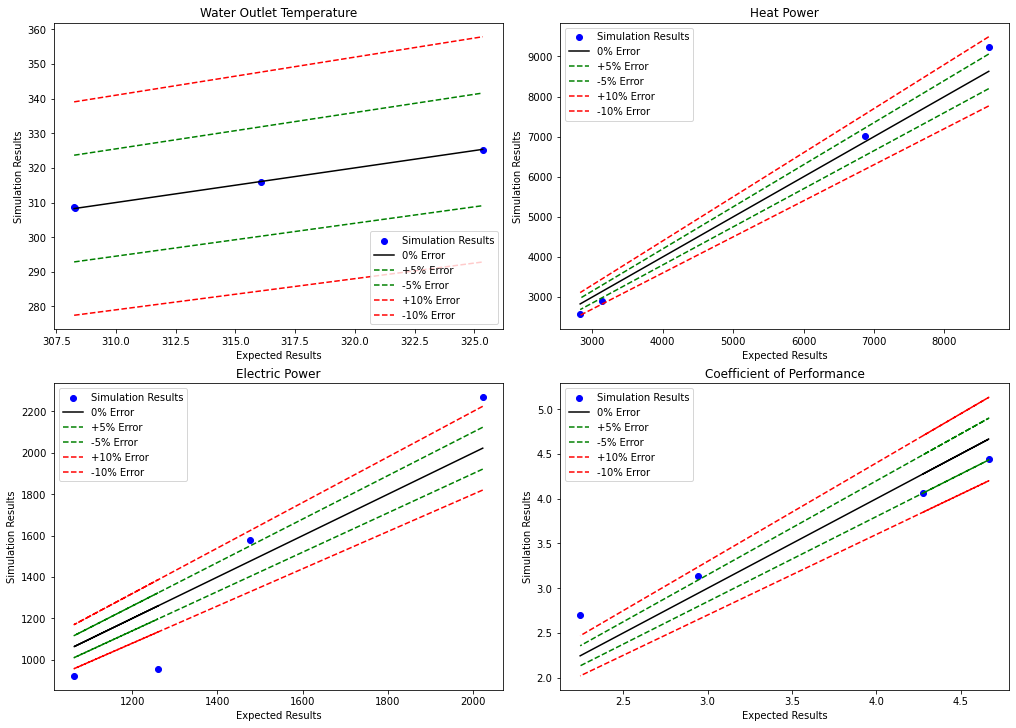
\includegraphics[width=\textwidth]{images/output.png}
    \caption{Percentage errors in Water Outlet Temperature, Heat Power, Electrical Power, and Coefficient of Performance between simulation and expected results.}
    \label{fig:percentage_errors}
\end{figure}

\section{Conclusion}

In conclusion, while our calibration methods have shown promise, especially with the PSO algorithm yielding tangible results, our journey encountered significant challenges. Notably, we aimed to incorporate an uncertainty analysis using OPENTURNS to enhance our calibration process further. Such an analysis would have been instrumental in identifying which performance indices were most sensitive to parameter variations, thus allowing us to focus our efforts more efficiently. Unfortunately, due to unforeseen computer bugs and the constraints of time, we were unable to implement this aspect of our study. This limitation prevented us from potentially achieving a more targeted and effective calibration process.

Despite this setback, it's important to highlight the achievements made. The PSO algorithm, in particular, has proven to be effective, albeit with room for further refinement. The calibration process, which processed all lines of heat pump data, was an exhaustive task. It took approximately 10 hours, with a swarm size of 8 and a maximum of 18 iterations, to complete. This underscores the intensive computational effort required but also points to the potential for optimizing these processes further.

Although the NSGA-II algorithm did not meet our expectations in terms of effectiveness, the experience gained from employing these diverse calibration methods has been invaluable. Moving forward, it would be beneficial to address the technical issues encountered with OPENTURNS and to continue refining our calibration approach. By doing so, we can enhance the accuracy and reliability of our simulations, ultimately contributing to more efficient and effective heat pump system designs.

% \phantomsection
\printbibliography
% \addcontentsline{toc}{chapter}{Bibliography}


\end{document}